%
% This file is part of AutoMATiC.
% AutoMATiC -- Automatic code generation based on the MATLAB and 
% C languages.
% 
% Copytight (C) 2018-2019 by Patryk Chaber. Developed within the 
% Warsaw University of Technology, Institute of Control and 
% Computation Engineering under supervision of Maciej Lawrynczuk. 
% All rights reserved.
% 
% AutoMATiC is free software: you can redistribute it and/or modify
% it under the terms of the GNU General Public License as published by
% the Free Software Foundation; either version 3 of the License, or
% (at your option) any later version.
% 
% AutoMATiC is distributed in the hope that it will be useful,
% but WITHOUT ANY WARRANTY; without even the implied warranty of
% MERCHANTABILITY or FITNESS FOR A PARTICULAR PURPOSE.  See the
% GNU General Public License for more details.
% 
% You should have received a copy of the GNU General Public License
% along with AutoMATiC.  If not, see <https://www.gnu.org/licenses/>.
%

\documentclass[a4paper,titlepage,11pt,twosides,floatssmall]{article}
\usepackage[left=2.5cm,right=2.5cm,top=2.5cm,bottom=2.5cm]{geometry}
\usepackage[OT1]{fontenc}
\usepackage{amsmath}
\usepackage{amsfonts}
\usepackage{amssymb}
\usepackage{graphicx}
\usepackage{url}
\usepackage{tikz}
\usetikzlibrary{arrows,calc,decorations.markings,math,arrows.meta}
\usepackage{rotating}
\usepackage[percent]{overpic}
\usepackage[cp1250]{inputenc}
\usepackage{xcolor}
\usepackage{pgfplots}
\usetikzlibrary{pgfplots.groupplots}
\usetikzlibrary{backgrounds}
\usepackage{listings}
\usepackage{matlab-prettifier}
\usepackage{enumitem,amssymb}
\definecolor{szary}{rgb}{0.95,0.95,0.95}
\usepackage{siunitx}
\sisetup{detect-weight,exponent-product=\cdot,output-decimal-marker={,},per-mode=symbol,binary-units=true,range-phrase={-},range-units=single}
\frenchspacing

\pgfplotsset{
	compat=newest,
	tick label style={font=\tiny},
	label style={font=\scriptsize},
	legend style={font=\scriptsize,draw=none,fill=none},
	title style={font=\scriptsize},
	xticklabel style={/pgf/number format/fixed}
}

\SendSettingsToPgf
%konfiguracje pakietu listings


\lstset{
	escapeinside = {@}{@},
	breaklines=true,
	tabsize=2,
	captionpos=t,
	xleftmargin=2pt,
	showstringspaces=false,
	aboveskip=0em,
  belowskip=0em,
  basicstyle=\footnotesize\ttfamily,
}

\lstdefinestyle{customlatex}{
	basicstyle=\footnotesize\ttfamily,
	%basicstyle=\small\ttfamily,
}

\definecolor{matlabtext}{HTML}{000000}
\definecolor{matlabbg}{HTML}{FFFFFF}
\definecolor{matlabkeywords}{HTML}{0000FF}
\definecolor{matlabcomments}{HTML}{228B22}
\definecolor{matlabstring}{HTML}{A020F0}
\definecolor{matlaberror}{HTML}{FF0000}
\definecolor{matlabvariable}{HTML}{000000}


\newlength\figureheight
\newlength\figurewidth
\setlength\figureheight{7cm}
\setlength\figurewidth{14cm}

\definecolor{myred}{rgb}{1.00000,0.00000,0.00000}%
\definecolor{mygreen}{rgb}{0.00000,0.70000,0.00000}%
\definecolor{myblue}{rgb}{0.00000,0.00000,1.00000}%
\definecolor{mydarkblue}{rgb}{0.00000,0.00000,0.70000}%
\definecolor{mylightblue}{rgb}{0.50000,0.50000,1.00000}%
\definecolor{mydarkred}{rgb}{0.70000,0.00000,0.00000}%
\definecolor{mydarkgreen}{rgb}{0.00000,0.50000,0.00000}%
\definecolor{myblack}{rgb}{0.00000,0.00000,0.00000}%
\definecolor{mycolor5}{rgb}{1.00000,0.95000,0.90000}%
\definecolor{mycolor6}{rgb}{0.90000,0.95000,1.00000}%

\newcommand{\unone}{$u$}
\newcommand{\uone} {$u_1$}
\newcommand{\utwo} {$u_2$}
\newcommand{\uthree} {$u_3$}
\newcommand{\uavg} {$\overline{u}$}
\newcommand{\ynone}   {$y$}
\newcommand{\yone}    {$y_1$}
\newcommand{\ytwo}    {$y_2$}
\newcommand{\ythree}    {$y_3$}
\newcommand{\yzadnone}{$y^\mathrm{sp}$}
\newcommand{\yzadone} {$y^\mathrm{sp}_1$}
\newcommand{\yzadtwo} {$y^\mathrm{sp}_2$}

\newcommand{\xstart}{0.5}

\newcommand{\plotthissiet}[1]{\begin{tikzpicture}
\begin{groupplot}[
    group style={
        group name=left plots,
        group size=1 by 2,
        vertical sep=15pt,
        x descriptions at=edge bottom},
    width=\figurewidth,
    height=\figureheight,
%    scale only axis,
    xmin=\xstart,
    xmax=50,
    axis background/.style={fill=white},
    legend pos=south east,legend columns=4,legend cell align={left},legend style={draw=none},
%    scale only axis
    ]
\nextgroupplot[%
xticklabels={,,},
ymin=-0.5,
ymax=0.5,
ylabel={\yone, \ytwo},
]
\addplot[thick,opacity=0.5,           color=myblue           ] % Y1
table[col sep = comma, x index = {0}, y index = {1}]{./#1.csv};
\addplot[thick,opacity=0.5,           color=myred     ,      ] % Y2
table[col sep = comma, x index = {0}, y index = {2}]{./#1.csv};
\addplot[thick,            const plot,color=mydarkblue,dashed] % Z1
table[col sep = comma, x index = {0}, y index = {3}]{./#1.csv};
\addplot[thick,            const plot,color=mydarkred ,dashed] % Z2
table[col sep = comma, x index = {0}, y index = {4}]{./#1.csv};
\legend{\yone,\ytwo,\yzadone,\yzadtwo};
\nextgroupplot[%
xlabel={time [s]},
ymin=-0.5,
ymax=0.5,
ylabel={\uone, \utwo},
]
\addplot[thick,opacity=0.5,const plot,color=myblue    ,      ] % U1
table[col sep = comma, x index = {0}, y index = {5}]{./#1.csv};
\addplot[thick,opacity=0.5,const plot,color=myred     ,      ] % U2
table[col sep = comma, x index = {0}, y index = {6}]{./#1.csv};
\legend{\uone,\utwo};
\end{groupplot}
\end{tikzpicture}%
}

\lstdefinestyle{myc}{
	language=C,
	backgroundcolor=\color{white},
	keywordstyle=\bfseries\color{green!40!black},
	commentstyle=\itshape\color{purple!40!black},
	identifierstyle=\color{blue},
	stringstyle=\color{orange},
	classoffset=1,% starting a new class
%	alsoletter=\#,
	otherkeywords={\#MPC\_BEGIN, \#MPC\_END, \#MPC\_INCLUDE, \#MPC\_PROFILER\_BEGIN, \#MPC\_PROFILER\_COUNT, \#MPC\_PROFILER\_END, \#MPC\_PROFILER\_PRINT},	
	morekeywords=[2]{\#MPC\_BEGIN,\#MPC\_END},
	keywordstyle=[2]\bfseries\color{orange},
	morekeywords=[3]{\#MPC\_PROFILER\_BEGIN, \#MPC\_PROFILER\_COUNT, \#MPC\_PROFILER\_END, \#MPC\_PROFILER\_PRINT},
	keywordstyle=[3]\bfseries\color{purple},
	morekeywords=[4]{\#MPC\_INCLUDE},
	keywordstyle=[4]\bfseries\color{red}, % not used anymore	
	morekeywords=[5]{CurrentControlPtr,CurrentControl},
	keywordstyle=[5]\bfseries\color{green!50!blue}, % not used anymore	
	morekeywords=[6]{ArchiveDataPtr,ArchiveData},
	keywordstyle=[6]\bfseries\color{green!50!red}, % not used anymore	
%	moredelim=**[is][\color{myred}]{@}{@},
}
\lstdefinestyle{mym}{
	language=matlab,
	backgroundcolor=\color{white},
	basicstyle=\footnotesize\ttfamily\color{matlabtext},
	keywordstyle=\bfseries\color{matlabkeywords},
	commentstyle=\color{matlabcomments},
	morecomment=[l][\color{matlabcomments}\bfseries]{\%\%},
	morecomment=[l][\color{matlabcomments}]{...},
	identifierstyle=\color{matlabvariable},
	stringstyle=\color{matlabstring},
}

%wymiar tekstu (bez �ywej paginy)
\textwidth 160mm \textheight 247mm

%ustawienia pakietu pgfplots
\pgfplotsset{
tick label style={font=\scriptsize},
label style={font=\small},
legend style={font=\small},
title style={font=\small}
}

\newcommand{\AutomaticMPC}{{\scshape AutoMATiC}}

\title{\bf\AutomaticMPC: Code Generation of Model Predictive Control Algorithms for Microcontrollers -- Tutorial for the User}
%\author{Patryk Chaber}
\date{\today}

\begin{document}
\maketitle

\tableofcontents
\newpage
\section{Introduction}
%{\color{red}W pracy wyslanej do recenzji nie ma podanych autorow, czy nalezy podac autora tutoriala? Czy wiec cytujemy prace wyslana do recenzji?}

%{\color{red}Czy w tytulach roz. 6 i 7 konieczne jest dodanie ,,Using one Microcontroller''? Pracy wieloprocesorowej nie rozwazamy. Ja bym skasowal.}

%{\color{red}Profiler, roz. 6.7: czy nie nalezy podac do czego odnosza sie poszczegolne id w tabelce?}

%{\color{red}Czy w tytule roz. 6.4 nie powinno byc Interrupts zamiast Interruptions?}

This tutorial describes how the \AutomaticMPC\ software system should be used in order to generate the C code of software implementation of Model Predictive Control (MPC) algorithms \cite{Camacho1999,Maciejowski2002,Tatjewski2007} for a chosen target microcontroller. Multiple-Input Multiple-Output (MIMO) processes are considered with $n_{\text{u}}$ manipulated variables (process inputs) $u_1,\ldots, u_{n_{\text{u}}}$ and $n_{\text{y}}$ controlled variables (process outputs) $y_1,\ldots, y_{n_{\text{y}}}$. In general, in MPC, at each discrete sampling instant, $k=0,1,\ldots$, the increments of the future manipulated variables (a vector of length $n_{\text{u}}N_{\text{u}}$) are repeatedly calculated on-line
\begin{equation}
\triangle\boldsymbol{u}(k)=\left[
\begin{array}
[c]{c}
\triangle u(k|k)\\
\vdots\\
\triangle u(k+N_{\text{u}}-1|k)
\end{array} 
\right]
\label{w_dUk}
\end{equation}
where $\triangle u(k+p|k)$ are backward differences of the manipulated variables for the future sampling instant $k+p$ calculated at the current instant $k$, $N_{\text{u}}$ is the control horizon. When calculation is completed, only the control increments for the current sampling instant are applied to the process. In the consecutive sampling instants process output variables are measured and the optimization procedure is repeated.

Two versions of MPC algorithms are available: analytical and numerical. In the first case the objective of MPC is to minimise the cost-function
\begin{align}
J(k)&=\sum_{p=1}^{N} \left\| y^{\text{sp}}(k+p|k)-\hat{y}(k+p|k) \right
\|^{2}_{\boldsymbol{\Psi}_0}+\sum_{p=0}^{N_{\text{u}}-1} \left\| \triangle u(k+p|k) \right\|^{2}_{\boldsymbol{\Lambda}_0}\label{w_Jk}
\end{align}
Its first part measures future control errors over the prediction horizon $N$, the second one is a penalty function used to minimize increments of the manipulated variables. $y^{\text{sp}}(k+p|k)$ and $\hat{y}(k+p|k)$ denote the vectors (of length $n_{\text{y}}$) of set-points and predicted values for the future sampling instant $k+p$ know at the instant $k$, $\boldsymbol{\Psi}_0=\text{diag}(\psi_1,\ldots,\psi_{n_{\text{y}}})$ and $\boldsymbol{\Lambda}_0=\text{diag}(\lambda_1,\ldots,\lambda_{n_{\text{u}}})$ are weighting matrices of dimensionality $n_{\text{y}}\times n_{\text{y}}$ and $n_{\text{u}}\times n_{\text{u}}$, respectively. The increments of the manipulated variables are calculated analytically, using computationally simple formulas \cite{Chaber2019}. The calculated signals are nex`t projected onto the admissible set determined by the constraints imposed on the values of the manipulated variables for the current sampling instant $k$ and the corresponding increments
\begin{align}
&u^{\min}\le u(k) \le u^{\max}\\
&-\triangle u^{\max} \le \triangle u(k) \le \triangle u^{\max}\label{w_ograniczenia_alg_analityczne}
\end{align}
where $u^{\min}$, $u^{\max}$ and $\triangle u^{\max}$ (the vectors of length $n_{\text{u}}$) denote minimal and maximal values as well as the maximal change of the manipulated variables, respectively.

In the case of the numerical MPC algorithms, at each sampling instant $k$, the full vector of future control increments (\ref{w_dUk}) is calculated as the solution of the following rudimentary MPC optimisation problem
\begin{align}
&\min\limits_{\triangle\boldsymbol{u}(k)} \left \{ J(k)\right \}\nonumber\\
&\text{subject to}\label{w_zad_opt_ogolnie}\\
&u^{\min} \leq u(k+p|k)\leq u^{\max},\ p=0,\ldots,N_{\text{u}}-1\nonumber\\
&-\triangle u^{\max} \leq\triangle
u(k+p|k)\leq\triangle u^{\max},\ p=0,\ldots
,N_{\text{u}}-1\nonumber
\end{align}
Provided that a linear model is used for prediction, i.e. to calculated the vectors $\hat{y}(k+p|k)$ for $p=1,\ldots,N$, numerical MPC algorithms result in quadratic optimisation. The OSQP \cite{osqp} library is used for quadratic optimisation in the \AutomaticMPC\ system.



Two MPC algorithms are available: Dynamic Matrix Control (DMC) \cite{Cutler1980} and Generalized Predictive Control (GPC) \cite{Clarke1987}, each of them in analytical and numerical versions. The DMC algorithm uses for prediction a simple to obtain step-response model of the controlled process. Provided that the process is stable with no integration, the model is comprised by $D$ (which is called the horizon of process dynamics) MIMO step-response matrices
\begin{equation}
\boldsymbol{S}_1, \boldsymbol{S}_2, \boldsymbol{S}_3, \ldots, \boldsymbol{S}_{\text{D}} \label{w_Sp}
\end{equation}
where the matrices of dimensionality $n_{\text{y}} \times n_{\text{u}}$ are
\begin{equation}
\boldsymbol{S}_p=\left[
\begin{array}
[c]{ccc}
s_p^{1,1} & \ldots & s_p^{1,n_{\text{u}}}\\
\vdots & \ddots & \vdots\\
s_p^{n_{\text{y}},1} & \ldots &  s_p^{n_{\text{y}},n_{\text{u}}}
\end{array}
\right] \label{w_Sp_struktura}
\end{equation}
The scalar step-response coefficient for the sampling instant $p$, the input $u_n$ and the output $y_m$ is denoted by $s_p^{m,n}$. The GPC algorithms uses the following difference equation model \cite{Chaber2019}
\begin{equation}
\boldsymbol{A}(q^{-1})y(k)=\boldsymbol{B}(q^{-1})u(k)\label{w_Ayk_Buk}
\end{equation}
where the entries of the matrices
\begin{align}
\boldsymbol{A}(q^{-1})&=\left[
\begin{array}
[c]{ccc}
A_{1,1}(q^{-1}) & \ldots & 0\\
\vdots & \ddots & \vdots\\
0 & \ldots & A_{n_{\text{y}},n_{\text{y}}}(q^{-1})
\end{array}
\right]\label{w_Aq1}\\
\boldsymbol{B}(q^{-1})&=\left[
\begin{array}
[c]{ccc}
B_{1,1}(q^{-1}) & \ldots & B_{1,n_{\text{u}}}(q^{-1})\\
\vdots & \ddots & \vdots\\
B_{n_{\text{y}},1}(q^{-1}) & \ldots & B_{n_{\text{y}},n_{\text{u}}}(q^{-1})
\end{array}
\right]\label{w_Bq1}
\end{align}
are the polynomials in the backward shift operator $q^{-1}$
\begin{equation}
A_{m,m}(q^{-1})=1+a_1^m q^{-1}+\ldots+a_{n_{\text{A}}}^m q^{-n_{\text{A}}}\label{w_Aii}
\end{equation}
for $m=1,\ldots,n_{\text{y}}$ and
\begin{equation}
B_{m,n}(q^{-1})=b_1^{m,n}q^{-1}+\ldots+b_{n_{\text{B}}}^{m,n}q^{-n_{\text{B}}}\label{w_Bij}
\end{equation}
for $m=1,\ldots,n_{\text{y}}$, $n=1,\ldots,n_{\text{u}}$.

%{\color{red}Skomentowac: w powyzszym opisie jest proces MIMO nu x ny, a w rozdziale ,,Communication with PC using USART'' mowiny o tylko dwoch zmiennych.}
\newpage 
\section{Conditions of Using the \AutomaticMPC\ System}
%This file is part of AutoMATiC.

\begin{lstlisting}
AutoMATiC -- Automatic code generation based on the MATLAB and 
C languages.

Copytight (C) 2018-2019 by Patryk Chaber. Developed within the 
Warsaw University of Technology, Institute of Control and 
Computation Engineering under supervision of Maciej Lawrynczuk. 
All rights reserved.

AutoMATiC is free software: you can redistribute it and/or modify
it under the terms of the GNU General Public License as published by
the Free Software Foundation; either version 3 of the License, or
(at your option) any later version.

AutoMATiC is distributed in the hope that it will be useful,
but WITHOUT ANY WARRANTY; without even the implied warranty of
MERCHANTABILITY or FITNESS FOR A PARTICULAR PURPOSE.  See the
GNU General Public License for more details.

You should have received a copy of the GNU General Public License
along with AutoMATiC.  If not, see <https://www.gnu.org/licenses/>.
\end{lstlisting}

\AutomaticMPC\ is open-source software, so you can use it free of charge under the terms of the GNU GPL licence. If you are using the software in your 
research work, you are supposed to cite one or more of the following references.

\begin{lstlisting}[escapeinside = {},]
@MISC{AutoMATiCTutorial,
  author = {P. Chaber},
  title = {{AutoMATiC} {T}utorial},
  howpublished = {https://github.com/pjchaber/automatic-mpc},
  year = {2019}
}

@ARTICLE{Chaber2019,
	author = {P. Chaber and M. \L{}awry\'{n}czuk},
	title = {{AutoMATiC}: Code Generation of Model Predictive Control Algorithms for Microcontrollers},
	note = {in review}
}
\end{lstlisting}

%{\color{red}Do napisania (na sieci sa generatory). Trzeba zdefiniowac czy uzytkownik ma prawo modyfikowac kody zrodlowe. Trzeba zdefiniowac co mozna uzytkownikowi niekomercyjnemu, a co komercyjnemu. Zlecic cytowanie artykulu z IEEE TII. Napisac, ze autor nie jest odpowiedzialny za zle dzialanie, ani za ew. szkody. 

%Ja bym zezwolil uzytkownikowi niekomercyjnemu na uzywanie i modyfikowanie. Chyba licencja Creative Commons jest zbyt liberalna.}

\section{Requirements}
This software was tested using following setup:
\begin{itemize}
\item Microsoft Windows 10 Pro
\item MATLAB 2019a
\item MinGW64 Compiler (C++)
\end{itemize}
and for the programming of the example microcontroller:
\begin{itemize}
\item STM32F746IGT6 microcontroller (part of the Core7XXI evaluation board with Open7XXI-C board -- both produced by WaveShare)
\item J-Link v9.3
\item Keil uVision v5.17.0.0
\item STM32CubeMX
\end{itemize}

Despite aforementioned configuration, this software was also tested with MATLAB 2017b, thus should work with any other MATLAB version in between of those two. This software should work also on Linux based operating systems, but it may require minor changes in paths notation.

\section{Installation}
To build \AutomaticMPC\ system compile its sources using \lstinline[style=mym]{mex} compiler in MATLAB with the following steps:
\begin{enumerate}
\item download or clone the repository of \AutomaticMPC:\\ \url{https://github.com/pjchaber/automatic-mpc.git}
\item make sure that MATLAB is callable from the shell by executing: \label{it:shell}
\begin{lstlisting}[]
matlab -batch "disp(version);"
\end{lstlisting}
which should print output similar to the following:
\begin{lstlisting}[]
9.6.0.1072779 (R2019a)
\end{lstlisting}
If the output differs, make sure that the following MATLAB directory:
\begin{lstlisting}[]
<MATLAB root directory>\bin\win64
\end{lstlisting}
is listed in \lstinline|PATH| variable of your system. For example:
\begin{lstlisting}[]
E:\Program Files\MATLAB\R2019a\bin\win64
\end{lstlisting}
\item register MATLAB for further use of its engine executing of the following instruction in shell:\label{it:regserver}
\begin{lstlisting}[]
matlab -regserver
\end{lstlisting}
\item change current working directory to a directory with the source of the project 
\item execute in MATLAB following instruction
\begin{lstlisting}[style=mym]
mex -v -client engine main.cpp XGetOpt.cpp -output automatic_transcompiler.exe;
\end{lstlisting}
If the compilation fails, make sure that you have set a C++ compiler by executing in MATLAB:
\begin{lstlisting}[style=mym]
mex -setup C++
\end{lstlisting}
Also make sure to use the same MATLAB version which was used in the shell in steps \ref{it:shell} and \ref{it:regserver}.
\end{enumerate}

The \AutomaticMPC\ system comes with already cloned version of OSQP (0.5.0), with a temporary minor bug fix (\url{https://github.com/oxfordcontrol/osqp/issues/157}). The cloned OSQP project was made following the instructions on \url{https://osqp.org/docs/get_started/sources.html#build-from-sources}, with additional call for \lstinline|cmake| right before the compilation:
\begin{lstlisting}
cmake -DPRINTING=OFF -DPROFILING=OFF -DCTRLC=OFF -DDFLOAT=ON -DENABLE_MKL_PARDISO=OFF .
\end{lstlisting}

\section{Setup}
All further examples focus on the task of controlling output voltages of emulated process. All signals used to connect the controller and the process are voltage signals of range from 0 to 3.3V. From the implementation side, those signals are represented as values from -1 to 1, where the lowest value represents 0V and the highest one represents 3.3V. The process that is emulated is a matrix of single inertia transfer functions (\ref{eq:obj}). Although the theoretical introduction considers any number of input and output signals, further on a process with only two inputs and two outputs is used. The process is configured exactly the same as the controller and utilises the same microcontroller to perform its tasks. Two ADC inputs of the controller are connected directly to the two DAC outputs of the process and two ADC inputs of the process are connected to the two DAC outputs of the controller, as shown in Fig. \ref{fig:setup}.

\begin{figure}
\centering
\includegraphics[width=\textwidth,page=12]{rysunki2}
\caption{Microcontrollers representing the MPC controller (1) and the emulated process (2) with their corresponding ADC and DAC connection pins (3) and (4), respectively}
\label{fig:setup}
\end{figure}

\section{Generation of a Single MPC}

Firstly, let us create the STM32CubeMX project which will be used as a base for further definition of a target platform's configuration (it is expected from the reader to know how to use STM32CubeMX and how to create projects for STM32F746IGT6 or similar and how to, based on such a project, generate a Keil uVision 5 project). Details of this project are as follows:
\begin{itemize}
	\item Target Platform: STM32F746IGTx
	\item Pinout and Configuration:
	\begin{itemize}
		\item RCC (HSE as Crystal/Ceramic Resonator)
		\item ADC3 (IN0 and IN1 enabled):
		\begin{itemize}
			\item Clock Prescaler: PLCK divided by 4
			\item Scan Conversion: Enabled
			\item Continuous Conversion: Enabled
			\item DMA Continuous Requests: Enabled
			\item Number of Regular Conversions: 2
			\item Rank 1:
			\begin{itemize}
				\item Channel: Channel 0
				\item Sampling Time: 144 Cycles
			\end{itemize}
			\item Rank 2:
			\begin{itemize}
				\item Channel: Channel 1
				\item Sampling Time: 144 Cycles
			\end{itemize}
		\end{itemize}
		\item DAC (OUT1 and OUT2 enabled), for both outputs:
		\begin{itemize}
			\item  Output Buffer: Enable
			\item  Trigger: None
		\end{itemize}
		\item TIM2 (Clock Source: Internal Clock):
		\begin{itemize}
			\item Prescaler: 1000-1
			\item Counter Period: 10800
		\end{itemize}
		\item TIM5 (Clock Source: Internal Clock):
		\begin{itemize}
			\item Prescaler: 0
			\item Counter Period: 0xffffffff
		\end{itemize}
		\item USART1 (Asynchronous):
		\begin{itemize}
			\item Data Direction: Transmit Only
		\end{itemize}
		\item DMA2
		\begin{itemize}
			\item ADC3:
			\begin{itemize}
				\item Stream: DMA2 Stream 0
				\item Direction: Peripheral to Memory
				\item Priority: Low
				\item Mode: Circular
				\item Peripheral Data Width: Word
				\item Memory Data Width: Word
			\end{itemize}
			\item ADC3:
			\begin{itemize}
				\item Stream: DMA2 Stream 0
				\item Direction: Peripheral to Memory
				\item Priority: Low
				\item Mode: Circular
				\item Peripheral Data Width: Word
				\item Memory Data Width: Word
			\end{itemize}
		\end{itemize}
		\item NVIC:
		\begin{itemize}
			\item Time base of System tick Timer (Preemption Priority: 5)
			\item ADC1, ADC2 and ADC3 global interrupts (Enable, Preemption Priority: 3)
			\item TIM2 global interrupts (Enabled, Preemption Priority: 1)
			\item USART1 global interrupts (Enabled)
			\item DMA2 stream0 global interrupts (Preemption Priority: 4)
		\end{itemize}
		\item RNG (Activated)
	\end{itemize}
	\item Clock Configuration:
	\begin{itemize}
		\item Input Frequency for HSE: 8Hz
		\item PLL Source Mux: HSE
		\item HCLK (MHz): 216 (confirm by pressing ENTER)
	\end{itemize}
	\item Project Manager:
	\begin{itemize}
		\item Toolchain / IDE: MDK-ARM V5
		\item Minimum Heap Size: 0x8000
		\item Minimum Stack Size: 0x40000
	\end{itemize}
\end{itemize}

After generating code to a Keil uVision 5 project communication interface with the PC and interface to connect process of control has to be implemented. It is worth making sure that all the code added to the project after its generation is placed between comments \lstinline[style=myc]|/* USER CODE BEGIN <name> */| and \lstinline[style=myc]|/* USER CODE END <name> */| which will further on be denoted as "\textless name\textgreater" block. It will further ease the process of regeneration of the microcontroller's configuration.

\subsection{Communication with PC using USART}
Firstly, in the \lstinline[]|main.c| file, \lstinline|string.h| library header has to be included in the "Includes" block. This will allow to send text messages to a PC in a simple manner. Next a simple wrapper for transmitting of a string should be defined in block "0":
\begin{lstlisting}[style=myc]
void write_string(char * txt){
	while(HAL_UART_GetState(&huart1) == HAL_UART_STATE_BUSY_TX);
	if(HAL_UART_Transmit_IT(&huart1, (uint8_t*)txt, strlen(txt))!= HAL_OK) 
		Error_Handler();  
	while(HAL_UART_GetState(&huart1) == HAL_UART_STATE_BUSY_TX);
}
\end{lstlisting}

At this point, it is possible to send text messages to a PC, it is worth noting that the new line character and carriage return is not included by default in the sent string.

All further controllers will send to a PC a message, at each sampling instant, in the following format \lstinline|x = [<y1>,<y2>,<z1>,<z2>,<u1>,<u2>,<alg>,];|, where the consecutive placeholders are defined as following:
\begin{itemize}
\item \lstinline|<y1>| -- the measurement of the first output signal,
\item \lstinline|<y2>| -- the measurement of the second output signal,
\item \lstinline|<z1>| -- the set point for the first output signal,
\item \lstinline|<z2>| -- the set point for the second output signal,
\item \lstinline|<u1>| -- the first control signal applied to a controlled process,
\item \lstinline|<u2>| -- the second control signal applied to a controlled process,
\item \lstinline|<alg>| -- the number of the algorithm used in the controller (used only when more than one control algorithm is used).
\end{itemize}
This format is convenient because messages that follows this format can be used in the MATLAB script as an argument of the \lstinline[style=mym]|eval| function and further easily plotted and saved as a CSV file.

\subsection{Measurement of Voltage Signals}
Voltage signals after conversion to a digital values will be averaged over 100 consecutive samples. Therefore a table for those raw measurements have to be defined in block "PV" as:
\begin{lstlisting}[style=myc]
uint32_t adc_val_raw[ADC_SIZE*2] = {0};
\end{lstlisting}
where \lstinline[style=myc]|ADC_SIZE| is defined in block "PD" as:
\begin{lstlisting}[style=myc]
#define ADC_SIZE 100
\end{lstlisting}
Due to having two signals, the size of table with raw measurements is \lstinline[style=myc]|ADC_SIZE*2|. To increase the resolution of averaged measurements, those will be stored as \lstinline[style=myc]|float| variables (block "PV"):
\begin{lstlisting}[style=myc]
float adc_val_f[2] = {0,0};
\end{lstlisting}

Having those defined, it is important to start a ADC unit. It can be implemented by inserting following code into a block "2":
\begin{lstlisting}[style=myc]
HAL_ADC_Start(&hadc3);
if(HAL_ADC_Start_DMA(&hadc3, (uint32_t*)adc_val_raw, ADC_SIZE*2) != HAL_OK) Error_Handler();
\end{lstlisting}

Thanks to a DMA mechanism, after obtaining 100 consecutive samples of each signal a specific callback function will be executed. It can be redefined to perform measurements' averaging as soon as they are available, by inserting following code in block "0":
\begin{lstlisting}[style=myc]
void HAL_ADC_ConvCpltCallback(ADC_HandleTypeDef* AdcHandle)
{
	static int i=0; 
	static uint32_t tmpval[2] = {0,0};
	for(i=0,tmpval[0]=0,tmpval[1]=0;i<ADC_SIZE; ++i){
		tmpval[0] += adc_val_raw[2*i];
		tmpval[1] += adc_val_raw[2*i+1];
	}
	adc_val_f[0] = ((float)tmpval[0]/ADC_SIZE-2047.5f)/2047.5f;
	adc_val_f[1] = ((float)tmpval[1]/ADC_SIZE-2047.5f)/2047.5f;
}
\end{lstlisting}
This will allow to have constant supply of averaged results from ADC without consuming much of a computational power of a microcontroller core (thanks to DMA).

\subsection{Creation of Voltage Signals}
To generate voltage signal DAC are used. Those are already configured thanks to the generation of the code from STM32CubeMX, although, they have to be started before they can be used. To start them, in the block "2" there has to be invoked:
\begin{lstlisting}[style=myc]
HAL_DAC_Start(&hdac, DAC_CHANNEL_1);
HAL_DAC_Start(&hdac, DAC_CHANNEL_2);
\end{lstlisting}
The following calls allow to generate 0V on first output and the 3.3V on the second one, since this is a 12 bit DAC:
\begin{lstlisting}[style=myc]
HAL_DAC_SetValue(&hdac, DAC1_CHANNEL_1,DAC_ALIGN_12B_R,0);
HAL_DAC_SetValue(&hdac, DAC1_CHANNEL_2,DAC_ALIGN_12B_R,4095);
\end{lstlisting}
and thus, to use this with a variable that ranges from -1 to 1, the following function is defined (in block "WHILE"):
\begin{lstlisting}[style=myc]
void __setControlValue(float* value){
  HAL_DAC_SetValue(&hdac, DAC1_CHANNEL_1,DAC_ALIGN_12B_R, (uint32_t)(value[0]*2047.5f+2047.5f));
  HAL_DAC_SetValue(&hdac, DAC1_CHANNEL_2,DAC_ALIGN_12B_R, (uint32_t)(value[1]*2047.5f+2047.5f));
}
\end{lstlisting}
where an array of two floats is an argument and it contains values for consecutive outputs.

\subsection{Induction of Interrupts with a Constant Frequency}
To generate an interrupt with a constant frequency which will further be used as an indicator of the beginning of new discrete sampling time, a timer TIM2 is used. It is already configured to generate events with a constant period of 100ms, but it is not started yet. To do so, the following code must be implemented in a block "2":
\begin{lstlisting}[style=myc]
HAL_TIM_Base_Init(&htim2);   
HAL_TIM_Base_Start_IT(&htim2);
\end{lstlisting}
This will cause an execution of a callback function which can be redefined:
\begin{lstlisting}[style=myc]
void HAL_TIM_PeriodElapsedCallback(TIM_HandleTypeDef *htim){
    if (htim->Instance == TIM2) {
		// interrupt each 100ms
    }
}
\end{lstlisting}
Although its implementation will be further extended.
\subsection{Interface for Further Ease of Use}
At this point it is worth to create additional functions that will wrap already existing functionality, so that anyone who will be working with this project in terms of control algorithms, will have easy interface to work with. Firstly, to give access to measurements signals the following will be used (block "0"):
\begin{lstlisting}[style=myc]
float* __measureOutput(){	
	return adc_val_f;
}
\end{lstlisting}
and it will return a pointer to a two element array of measurement values. It is clearly visible that it is analogous to the previously defined \lstinline[style=myc]|void __setControlValue(float* value)| function. Those two functions have to have their declarations in the header file corresponding to the source file in which they are defined (block "EFP" in \lstinline|main.h|). In this header, it could be convenient to declare also a function for communication with a PC \lstinline[style=myc]|void write_string(char * txt)|.

Because the main function of the program (namely \lstinline[style=myc]|int main(void)|) is defined in the \AutomaticMPC\ system software framework, the existing one have to be redefined using another name, e.g. \lstinline[style=myc]|void low_lvl_main(void)| which of course also has to be accessible from other source files. Therefore its declaration has to be given in a proper header file. It is also important to remove the \lstinline[style=myc]|while| loop from the \lstinline[style=myc]|low_lvl_main| function, so that it will not hang the controller.

At the end it will be convenient to set up the Keil uVision 5 project in such a way that the transcompilation process is executed always right before the build process starts. For this, "Options for Target" window has to be opened and in the "User" tab, in "Before Build/Rebuild" a "Run \#1" has to be filled with an execution of the transcompiler. The following will be used:
\begin{lstlisting}
<absolute path to AutoMATiC>/automatic_transcompiler.exe -I -p -c -i ../Src/main.mpc -o ../Src/main_mpc.c -l <absolute path to AutoMATiC>/Libs/MATLAB/ -L <absolute path to AutoMATiC>/Libs/C/
\end{lstlisting}
It is worth noting that the transcompiler is executed while being in the directory with a project file (i.e. \lstinline|MDK-ARM|). Consecutive arguments of the \lstinline|automatic_transcompiler.exe| execution denotes:
\begin{itemize}
\item \lstinline|-I| -- usage of the interrupt based software framework variant,
\item \lstinline|-p| -- usage of the profiler,
\item \lstinline|-c| -- usage of the forced delay of the control signal application,
\item \lstinline|-i <path>| -- relative path to the input file used for transcompilation,
\item \lstinline|-o <path>| -- relative path to the output file storing the result of transcompilation,
\item \lstinline|-l <path>| -- relative path to the directory with MATLAB libraries of the transcompiler,
\item \lstinline|-L <path>| -- relative path to the directory with C libraries of the transcompiler.
\end{itemize}

To complete the setup of the project one has to add source files and headers of \AutomaticMPC\ system to a project for further compilation. All these files can be found in a directory \lstinline|<absolute path to AutoMATiC>/Libs/C/|. Also a file named \lstinline|main.mpc| has to be created and placed in the \lstinline|../Src/| directory. This file will contain all the logic of the controller with as few low level implementation parts as possible. 

To incorporate OSQP solver one has to add a list of files into the Keil uVision5 project (it is best to create additional group for those files):
\begin{itemize}[itemsep=0pt]
\item \lstinline|<path to AutoMATiC>/Libs/C/osqp/src/auxil.c   |
\item \lstinline|<path to AutoMATiC>/Libs/C/osqp/src/cs.c      |
\item \lstinline|<path to AutoMATiC>/Libs/C/osqp/src/kkt.c     |
\item \lstinline|<path to AutoMATiC>/Libs/C/osqp/src/lin_alg.c |
\item \lstinline|<path to AutoMATiC>/Libs/C/osqp/src/lin_sys.c |
\item \lstinline|<path to AutoMATiC>/Libs/C/osqp/src/osqp.c    |
\item \lstinline|<path to AutoMATiC>/Libs/C/osqp/src/polish.c  |
\item \lstinline|<path to AutoMATiC>/Libs/C/osqp/src/proj.c    |
\item \lstinline|<path to AutoMATiC>/Libs/C/osqp/src/scaling.c |
\item \lstinline|<path to AutoMATiC>/Libs/C/osqp/src/util.c    |
\item \lstinline|<path to AutoMATiC>/Libs/C/osqp/lin_sys/direct/qdldl/qdldl_interface.c |
\item \lstinline|<path to AutoMATiC>/Libs/C/osqp/lin_sys/direct/qdldl/qdldl_sources/src/qdldl.c |
\item \lstinline|<path to AutoMATiC>/Libs/C/osqp/lin_sys/direct/qdldl/amd/src/amd_1.c              |
\item \lstinline|<path to AutoMATiC>/Libs/C/osqp/lin_sys/direct/qdldl/amd/src/amd_2.c              |
\item \lstinline|<path to AutoMATiC>/Libs/C/osqp/lin_sys/direct/qdldl/amd/src/amd_aat.c            |
\item \lstinline|<path to AutoMATiC>/Libs/C/osqp/lin_sys/direct/qdldl/amd/src/amd_control.c        |
\item \lstinline|<path to AutoMATiC>/Libs/C/osqp/lin_sys/direct/qdldl/amd/src/amd_defaults.c       |
\item \lstinline|<path to AutoMATiC>/Libs/C/osqp/lin_sys/direct/qdldl/amd/src/amd_info.c           |
\item \lstinline|<path to AutoMATiC>/Libs/C/osqp/lin_sys/direct/qdldl/amd/src/amd_order.c          |
\item \lstinline|<path to AutoMATiC>/Libs/C/osqp/lin_sys/direct/qdldl/amd/src/amd_post_tree.c      |
\item \lstinline|<path to AutoMATiC>/Libs/C/osqp/lin_sys/direct/qdldl/amd/src/amd_postorder.c      |
\item \lstinline|<path to AutoMATiC>/Libs/C/osqp/lin_sys/direct/qdldl/amd/src/amd_preprocess.c     |
\item \lstinline|<path to AutoMATiC>/Libs/C/osqp/lin_sys/direct/qdldl/amd/src/amd_valid.c          |
\item \lstinline|<path to AutoMATiC>/Libs/C/osqp/lin_sys/direct/qdldl/amd/src/SuiteSparse_config.c |
\end{itemize}
Also a following list of directories has to be included in the searching path:
\begin{itemize}[itemsep=0pt]
\item \lstinline|<path to AutoMATiC>/Libs/C/osqp/include/|
\item \lstinline|<path to AutoMATiC>/Libs/C/osqp/lin_sys/direct/qdldl/|
\item \lstinline|<path to AutoMATiC>/Libs/C/osqp/lin_sys/direct/qdldl/qdldl_sources/include/|
\item \lstinline|<path to AutoMATiC>/Libs/C/osqp/lin_sys/direct/qdldl/amd/include/|
\item \lstinline|<path to AutoMATiC>/Libs/C/osqp/lin_sys/|
\end{itemize}

\subsection{Logic of the Control Algorithm}
The file that contains logic of the controller, namely \lstinline|main.mpc|, contains implementations which can be divided in a few parts:
\begin{itemize}
\item utilisation of the low level interface functions,
\item invoke of the MATLAB script, used for automatic code generation of the MPC algorithm,
\item implementation of controllers behaviour.
\end{itemize}
The execution of the MATLAB script is not necessary -- content of this script could be as well placed right here. This notation nevertheless allows for clearer separation of the aforementioned parts of implementation of this file:

\begin{lstlisting}[style=myc]
#include "stm32f7xx_hal.h"
#include <string.h>
#include "main.h"

ArchiveData ad;
CurrentControl cc;

long get_time(){ return HAL_GetTick(); }

extern void timer_loop(void);
void HAL_TIM_PeriodElapsedCallback(TIM_HandleTypeDef *htim){
    if (htim->Instance == TIM2) {
        timer_loop();
    }
}
void measurements(){
    #MPC_PROFILER_BEGIN 4 @\color{myred}measurements@
    new_output(&ad,__measureOutput());
    #MPC_PROFILER_END 4
}
void controls(){
    #MPC_PROFILER_BEGIN 3 @\color{myred}controls' application@
    __setControlValue(last_control(&ad));
    #MPC_PROFILER_END 3
}
void hardware_setup(){
    #MPC_PROFILER_BEGIN 1 @\color{myred}hardware setup@
    low_lvl_main();
    #MPC_PROFILER_END 1
}

#MPC_BEGIN
\end{lstlisting}
\begin{lstlisting}[style=mym]
% Here is the MATLAB code
algorithms_parameters_definitions
\end{lstlisting}
\begin{lstlisting}[style=myc]
#MPC_END

void controller_setup(){
    #MPC_PROFILER_BEGIN 2 @\color{myred}software setup@
    init_archive_data(&ad, 200, 200, 2, 2, 0, 0, 0.01);
    init_current_control(&cc,&ad);
    controller(NULL,NULL);
    #MPC_PROFILER_END 2
}

void idle(){
    #MPC_PROFILER_BEGIN 13 @\color{myred}other procedures@
    const int k = 0;
	static char str[1000] = {0};

    sprintf(str, "x = [%f,%f,",ad.y[k][0], ad.y[k][1]);    write_string(str);
    sprintf(str,      "%f,%f,",ad.z[0], ad.z[1]);          write_string(str);
    sprintf(str,      "%f,%f,",ad.u[k-1][0],ad.u[k-1][1]); write_string(str);
    write_string("];\n\r");
	if(++i > 1000) {
		#MPC_PROFILER_PRINT
	}
    #MPC_PROFILER_END 13
}

void loop(){
    #MPC_PROFILER_BEGIN 10 @\color{myred}controls' calculation@
    static int i = 0;
	     if(i< 100){ ad.z[0] = -0.1f; ad.z[1] = +0.2f; }
	else if(i< 150){ ad.z[0] = -0.1f; ad.z[1] = -0.2f; }
	else if(i< 250){ ad.z[0] = +0.1f; ad.z[1] = -0.2f; }
	else           { ad.z[0] = +0.1f; ad.z[1] = +0.2f; }
	if(++i > 300) i = 0;
	
    #MPC_PROFILER_BEGIN 50 @\color{myred}control algorithm@
	controller(&ad,&cc);
	#MPC_PROFILER_END 50
	
    push_current_controls_to_archive_data(&cc,&ad);	
    #MPC_PROFILER_END 10		
}

void timeout(){
    while(1);
}
\end{lstlisting}

On the listing, there is a reference to a function called \lstinline[style=myc]|controller| which declaration is as follows:
\begin{lstlisting}[style=myc]
void controller(ArchiveData * ad, CurrentControl * c);
\end{lstlisting}
This function will be generated as soon as the MATLAB script is finished.

The \AutomaticMPC\ system software framework assumes that there is an implementation of functions:
\begin{itemize}
\item \lstinline[style=myc]|void write_string(char * str);| -- a function used by the profiler to write out the results of its measurements,
\item \lstinline[style=myc]|long get_time(void);|  -- a function used by the profiler to measure time of execution,
\item \lstinline[style=myc]|void hardware_setup(void);| -- a function used to setup hardware configuration of the controller,
\item \lstinline[style=myc]|void controller_setup(void);| -- a function used to setup software configuration of the controller,
\item \lstinline[style=myc]|void measurements(void);| -- a function used to obtain measurements for the current controller iteration,
\item \lstinline[style=myc]|void loop(void);| -- a function used to define the behaviour of the controller -- here control algorithms are executed,
\item \lstinline[style=myc]|void controls(void);| -- a function used to determine what to do with results obtained from the consecutive control algorithms,
\item \lstinline[style=myc]|void idle(void);| -- a function used for other, lower prioritized procedures,
\item \lstinline[style=myc]|void timeout(void);| -- a function executed when the calculation lasts longer than the sampling period.
\end{itemize}
These functions are used in the framework, in the predefined order. If some of these are not implemented, a default (often empty) implementation is assumed.

To implement interrupt based variant of the software framework, a function
\begin{lstlisting}[style=myc]
extern void timer_loop(void);
\end{lstlisting}
has to be declared and called each time a new discrete time instant starts. In these examples it occurs each time, the timer TIM2 generates an interrupt and thus causes execution of the following function:
\begin{lstlisting}[style=myc]
void HAL_TIM_PeriodElapsedCallback(TIM_HandleTypeDef *htim);
\end{lstlisting}

Each new measurement has to be stored in the \lstinline[style=myc]|ArchiveData| structure using
\begin{lstlisting}[style=myc]
void new_output(ArchiveDataPtr ad, float* y);
\end{lstlisting}
function. Also the final values of new control signals have to be stored in the same structure using 
\begin{lstlisting}[style=myc]
void push_current_controls_to_archive_data(CurrentControlPtr c,ArchiveDataPtr ad);
\end{lstlisting}
where \lstinline[style=myc]|CurrentControl| structure is filled by each control algorithm.

Lastly, there are a few functions in the \lstinline[style=myc]|void controller_setup()| function that are necessary to use those two structures. A function 
\begin{lstlisting}[style=myc]
void init_archive_data(ArchiveDataPtr ad, 
	long number_of_u, long number_of_y, 
	long size_of_u, long size_of_y, 
	float default_u, float default_y, 
	float current_yzad);
\end{lstlisting}
is used to initialize the \lstinline[style=myc]|ArchiveData| instance. The first argument is a pointer to this structure instance, next there are two parameters used to define number of control and output signals (in this order) of the process of control. Further there are two values that determine how many previous values of control and output signals have to be stored in the memory of the controller. Finally, there are default values of control, output and set-point signal, used for initialization of the microcontroller memory -- those can be changed as soon as the initialization function is finished.

Next function is
\begin{lstlisting}[style=myc]
void init_current_control(CurrentControlPtr cc, ArchiveDataPtr ad);
\end{lstlisting}
which is used to allocate memory for an instance of \lstinline[style=myc]|CurrentControl| based on the data stored in the alreaty setup \lstinline[style=myc]|ArchiveData| instance.

At the end of the software setup, there is an execution of the controller function, with both parameters set to \lstinline[style=myc]|NULL| which is used to initialize some values of the controller that are constant through its whole existence -- this will be clear as soon as the generated code of the algorithm appears.

\subsection{Dynamic Matrix Control Algorithm: Analytical version}
From this point on, only the \lstinline[style=myc]|algorithms_parameters_definitions.m| will be modified in order to generate software implementations of various control algorithms. It is important to make sure that this script is placed in the \lstinline|Src| directory of the Keil uVision 5 project. All further algorithms will be used to control output signals of the process described with the following example transfer function matrix:
\begin{equation}
G(s) = \left[\begin{array}{cc}
\displaystyle\tfrac{5}{0.14s+1} & \displaystyle\tfrac{1}{0.10s+1} \\[1mm]
\displaystyle\tfrac{1}{0.06s+1} & \displaystyle\tfrac{2}{0.08s+1} \\
\end{array}\right]\label{eq:obj}
\end{equation}
Based on this transfer function one can derive various discrete time models, specifically model in a form of step response coefficients (which is required by the DMC algorithm) or a set of difference equations (used in the GPC algorithm). First, one must create a continuous time transfer function in MATLAB:
\begin{lstlisting}[style=mym]
clear all
%% Process definition
Gs  = [... 
    tf(5,[.14,1]),tf(1,[.10,1]);...
    tf(1,[.06,1]),tf(2,[.08,1]);...
];               % continuous transfer function
\end{lstlisting}
It is worth to clear the workspace at the beginning of this script in order to avoid problems with accidental use of old variables. Next, this transfer function have to be transformed into a discrete time one and thus following have to be executed:
\begin{lstlisting}[style=mym]
Gz = c2d(Gs,0.1); % discrete transfer function
ny = 2; % number of output signals
nu = 2; % number of control signals
\end{lstlisting}
Additional definition of the number of output and control signals is just for the cleaner code in further part of this script. For the discretization, a sampling time of 0.1 s was used.

To determine step response coefficients a \lstinline[style=mym]|step| function of MATLAB could be used, but results would have to be modified in the convenient way. For the sake of clarity, this script does not utilize this function, it calculates this coefficients based on the GPC model instead. Therefore the ARX model used in GPC will be determined firstly:

\begin{lstlisting}[style=mym]
for m=1:2 % ARX model determination
    tmpa = conv(Gz.Den{m,1},Gz.Den{m,2}); GPC_a(m,:)   = tmpa(2:end);
    tmpb = conv(Gz.Num{m,1},Gz.Den{m,2}); GPC_b(m,1,:) = [tmpb(1:end) 0]; 
    tmpb = conv(Gz.Num{m,2},Gz.Den{m,1}); GPC_b(m,2,:) = [tmpb(1:end) 0];
end
\end{lstlisting}

This script cannot be used for a process with a different dimensionality -- a more general approach would be necessary. Next, the dynamics horizon is defined and the step response is obtained:
\begin{lstlisting}[style=mym]
D = 5;  % dynamics horizon
S = step_response_generation(GPC_a,GPC_b,D);
\end{lstlisting}
and the \lstinline[style=mym]|step_response_generation| is defined at the end of this script as follows:

\begin{lstlisting}[style=mym]
function S = step_response_generation(GPC_a,GPC_b,D)
    ny = size(GPC_a,1);
    nu = size(GPC_b,2);
    S = zeros(ny,nu,D);
    for k = 1:size(S,3)
        for m=1:ny
            for n=1:nu
                for i=1:min(k,size(GPC_b,3))
                    S(m,n,k) = S(m,n,k) + GPC_b(m,n,i)*1;
                end
                for i=1:min(k-1,size(GPC_a,2))
                    S(m,n,k) = S(m,n,k) - GPC_a(m,i)*S(m,n,k-i);
                end         
            end   
        end 
    end
    % adding a single iteration of delay
    S(:,:,2:end+1) = S(:,:,1:end); 
    S(:,:,1) = S(:,:,1)*0; 
end
\end{lstlisting}

Here, a set of general parameters of MPC algorithms is defined:
\begin{lstlisting}[style=mym]
% General control algorithms' parameters
N  = 5; % prediction horizon
Nu = 5; % control horizon
lambda= [1.0 1.0]; % Penalty--control signals' increments
psi   = [1.0 1.0]; % Penalty--control errors
dumin =-[.01 .01]; % Lower bound--control increments
dumax = [.01 .01]; % Upper bound--control increments
umin  =-[1.0 1.0]; % Lower bound--control signal
umax  = [1.0 1.0]; % Upper bound--control signal
\end{lstlisting}

and lastly, the automatic code generation procedure is called:
\begin{lstlisting}[style=mym]
AutoMATiC_Generate('AutoMATiC_DMC_Analytic_Algorithm','controller');
\end{lstlisting}
This function is defined in the script in \lstinline|<path to AutoMATiC>/Libs/MATLAB/|. Three arguments at most can be passed to this function, in the following order: the name of the algorithm which definition will be used to generate C code (it corresponds to the name of the script with an algorithm definition -- these can be found in the \lstinline|<path to AutoMATiC>/Libs/MATLAB/| directory), the name of the generated C function and a binary logic value which defines if there will be more algorithms generated in the same MATLAB script. The meaning of the last parameter will be clear in the example where two algorithms are generated for one controller project. 

At this point, if the build procedure will be called on the Keil uVision5 project, the automatic code generation will be called first which will generate a file called \lstinline|main_mpc.c| which can be found in Appendix \ref{ch:dmca}.

As it is visible, the \lstinline|<path to AutoMATiC>| in this example is \lstinline|C:\Users\Admin\Documents\GitHub\AutoMATiC|. It is worth noting that there is no part where the MATLAB code could be placed, instead there is a definition of the \lstinline[style=myc]|void controller(ArchiveData * ad, CurrentControl * c)| function. Also each pair of \lstinline[style=myc]|#MPC_PROFILER_BEGIN <id> <description>| and \lstinline[style=myc]|#MPC_PROFILER_END <id>| is substituted with a pair of corresponding C functions \lstinline[style=myc]|profiler_start(<id>,<description>)| and \lstinline[style=myc]|profiler_end(<id>)|, where \lstinline|<id>| is the identifier of the block, and the \lstinline|<description>| is the additional description of this block. Also a keyword \lstinline[style=myc]|#MPC_PROFILER_PRINT| is translated into a function \lstinline[style=myc]|profiler_print()| call, which prints out the current state of profiler using  \lstinline[style=myc]|write_string| function. If this generated C language source file is not included in the project and the build fails -- it is necessary to add this file to the project and repeat the building process. At this point everything should be ready to program the microcontroller and test the MPC controller itself.

\begin{figure}
\centering
\plotthissiet{dmca}
\caption{Trajectories of controlled and manipulated variables obtained when the analytical DMC controller is used}
\label{fig:dmca}
\end{figure}
A plot of signals measurements obtained from this controller is shown in Fig. \ref{fig:dmca}. Also the result generated with a profiler is shown in Table \ref{tab:dmca}. The consecutive columns in this and further shown tables are as follows:
\begin{itemize}
\item id -- the identifier of the block of code which was to be inspected (additional description in the parenthesis),
\item time total -- the total time that the program spent executing this block,
\item entries -- the number of times the program entered this block,
\item min -- the minimum amount of time spent executing this block,
\item mean -- the mean amount of time spent executing this block,
\item max -- the maximum amount of time spent executing this block,
\item running -- the flag denoting if this data was obtained during execution of this block (1 -- yes, 0 -- no).
\end{itemize}
All time measurements are obtained using the \lstinline[style=myc]|get_time| function, thus in this and following examples, their unit is a millisecond.

\begin{table}
\centering
\caption{Profiler results obtained when the analytical DMC controller is used}
\label{tab:dmca}
\begin{tabular}{ccccccc}
        id & time total &    entries &        min &       mean &        max &    running\\\hline
    1 (hardware setup) &          1 &          1 &          1 &     1.0000 &          1 & 0\\
    2 (software setup) &          1 &          1 &          1 &     1.0000 &          1 & 0\\
    3 (controls' application) &          8 &       1001 &          0 &     0.0079 &          1 & 0\\
    4 (measurements) &         59 &       1001 &          0 &     0.0589 &          1 & 0\\
   10 (controls' calculation) &        190 &       1001 &          0 &     0.1898 &          1 & 0\\
   50 (control algorithm) &         88 &       1001 &          0 &     0.0879 &          1 & 0\\
   13 (other procedures) &       7015 &       1001 &          6 &     7.0079 &          8 & 1\\
\end{tabular}
\end{table}

\subsection{Dynamic Matrix Control Algorithm: Numerical Version}
Based on the already created project for analytical version of DMC algorithm, a change to its numerical version is straightforward. It only requires the change od the name of used algorithm, i.e. the following line from the \lstinline|algorithms_parameters_definitions.m| script:
\begin{lstlisting}[style=mym]
AutoMATiC_Generate('AutoMATiC_DMC_Analytic_Algorithm','controller');
\end{lstlisting}
has to be changed to:
\begin{lstlisting}[style=mym]
AutoMATiC_Generate('AutoMATiC_DMC_Numeric_Algorithm','controller');
\end{lstlisting}
which, after performing same tasks as before to generate the final pure C code, will result in the code listed in Appendix \ref{ch:dmcn}.


\begin{figure}
\centering
\plotthissiet{dmcn}
\caption{Trajectories of controlled and manipulated variables obtained when the numerical DMC controller is used}
\label{fig:dmcn}
\end{figure}
A plot of signals measurements obtained from this controller is shown in Fig. \ref{fig:dmcn}. Also the result generated with a profiler is shown in Table \ref{tab:dmcn}.

\begin{table}
\centering
\caption{Profiler results obtained when the numerical DMC controller is used}
\label{tab:dmcn}
\begin{tabular}{ccccccc}
        id & time total &    entries &        min &       mean &        max &    running\\\hline
    1 (hardware setup) &          1 &          1 &          1 &     1.0000 &          1 & 0\\
    2 (software setup) &         13 &          1 &         13 &    13.0000 &         13 & 0\\
    3 (controls' application) &          0 &       1001 &          0 &     0.0000 &          0 & 0\\
    4 (measurements) &         66 &       1001 &          0 &     0.0659 &          1 & 0\\
   10 (controls' calculation) &       7415 &       1001 &          7 &     7.4075 &         43 & 0\\
   50 (control algorithm) &       7307 &       1001 &          7 &     7.2997 &         43 & 0\\
   13 (other procedures) &       6988 &       1001 &          6 &     6.9810 &          8 & 1\\
\end{tabular}
\end{table}

\subsection{General Predictive Control Algorithm: Analytical Version}
Due to the already performed determination of the GPC model in considered MATLAB script, only a simple modification has to be performed to change which algorithm is to be generated to a GPC in its analytical version. Therefore the line:
\begin{lstlisting}[style=mym]
AutoMATiC_Generate('AutoMATiC_DMC_Numeric_Algorithm','controller');
\end{lstlisting}
should be changed to:
\begin{lstlisting}[style=mym]
AutoMATiC_Generate('AutoMATiC_GPC_Analytic_Algorithm','controller');
\end{lstlisting}
which, after performing same tasks as before to generate the final pure C code, will result in the code listed in Appendix \ref{ch:gpca}.

\begin{figure}
\centering
\plotthissiet{gpca}
\caption{Trajectories of controlled and manipulated variables obtained when the analytical GPC controller is used}
\label{fig:gpca}
\end{figure}
A plot of signals measurements obtained from this controller is shown in Fig. \ref{fig:gpca}. Also the result generated with a profiler is shown in Table \ref{tab:gpca}.

\begin{table}
\centering
\caption{Profiler results obtained when the analytical GPC controller is used}
\label{tab:gpca}
\begin{tabular}{ccccccc}
        id & time total &    entries &        min &       mean &        max &    running\\\hline
    1 (hardware setup) &          1 &          1 &          1 &     1.0000 &          1 & 0\\
    2 (software setup) &          1 &          1 &          1 &     1.0000 &          1 & 0\\
    3 (controls' application) &          1 &       1001 &          0 &     0.0009 &          1 & 0\\
    4 (measurements) &         59 &       1001 &          0 &     0.0589 &          1 & 0\\
   10 (controls' calculation) &        164 &       1001 &          0 &     0.1638 &          1 & 0\\
   50 (control algorithm) &         58 &       1001 &          0 &     0.0579 &          1 & 0\\
   13 (other procedures) &       7026 &       1001 &          6 &     7.0189 &          8 & 1\\
\end{tabular}
\end{table}
\subsection{General Predictive Control Algorithm: Numerical Version}
Again, to change the analytical version of GPC algorithm to its numerical version, a change from:
\begin{lstlisting}[style=mym]
AutoMATiC_Generate('AutoMATiC_GPC_Analytic_Algorithm','controller');
\end{lstlisting}
to:
\begin{lstlisting}[style=mym]
AutoMATiC_Generate('AutoMATiC_GPC_Numeric_Algorithm','controller');
\end{lstlisting}
has to be performed. After performing same tasks as before to generate the final pure C code, will result in the code listed in Appendix \ref{ch:gpcn}.

\begin{figure}
\centering
\plotthissiet{gpcn}
\caption{Trajectories of controlled and manipulated variables obtained when the numerical GPC controller is used}
\label{fig:gpcn}
\end{figure}
A plot of signals measurements obtained from this controller is shown in Fig. \ref{fig:gpcn}. Also the result generated with a profiler is shown in Table \ref{tab:gpcn}.
\begin{table}
\centering
\caption{Profiler results obtained when the numerical GPC controller is used}
\label{tab:gpcn}
\begin{tabular}{ccccccc}
        id & time total &    entries &        min &       mean &        max &    running\\\hline
    1 (hardware setup) &          1 &          1 &          1 &     1.0000 &          1 & 0\\
    2 (software setup) &         13 &          1 &         13 &    13.0000 &         13 & 0\\
    3 (controls' application) &          0 &       1001 &          0 &     0.0000 &          0 & 0\\
    4 (measurements) &         64 &       1001 &          0 &     0.0639 &          1 & 0\\
   10 (controls' calculation) &       8691 &       1001 &          7 &     8.6823 &         44 & 0\\
   50 (control algorithm) &       8596 &       1001 &          7 &     8.5874 &         44 & 0\\
   13 (other procedures) &       6990 &       1001 &          6 &     6.9830 &          8 & 1\\
\end{tabular}
\end{table}

\section{Multiple MPC Algorithms Exchanged On-line in a Seamless Way Using One Microcontroller}
%\subsection{Analytical and Numerical Versions of DMC}
It is possible to implement the MPC controller which contains a number of different algorithms which are exchanged on-line in a seamless way. Let us consider an example in which two versions of the DMC algorithm are implemented, i.e. analytical and numerical. In such a case it is required to perform some minor changes both in the controllers' logic (\lstinline|main.mpc|) and the MATLAB script that defines parameters of used algorithms (\lstinline|algorithms_parameters_definitions.m|). In the logic part, a new global variable, e.g. \lstinline[style=myc]|int algorithm_used = 0;| should be created -- it will define which algorithm is currently used. Next, the switching logic should be implemented -- in the \lstinline[style=myc]|void loop()| function a simple condition will be added:
\begin{lstlisting}[style=myc]
if(algorithm_used == 0) controllerDMCA(&ad,&cc);
else                    controllerDMCN(&ad,&cc);
\end{lstlisting}
which will define that if the variable \lstinline[style=myc]|algorithm_used| equals 0, the analytical version of DMC algorithm will be used, otherwise a numerical version will be executed. It is also clearly visible that those algorithms have new, distinct names. These should be used consequently in both C and MATLAB code. All will be properly set further in this document. First, the software initialization function (named \lstinline[style=myc]|controller_setup|) has to be modified, by substituting a line:
\begin{lstlisting}[style=myc]
controller(NULL,NULL);
\end{lstlisting}
with two new lines:
\begin{lstlisting}[style=myc]
controllerDMCA(NULL,NULL);
controllerDMCN(NULL,NULL);
\end{lstlisting}
Lastly, the value of variable \lstinline[style=myc]|algorithm_used| has to be defined in time. Therefore, in the function \lstinline[style=myc]|loop()|, right before the newly added conditional execution of control algorithms, the following code should be added:
\begin{lstlisting}[style=myc]
if((i%10==0) && ((random() % 100) < 10))
	algorithm_used = algorithm_used==0?1:0;
\end{lstlisting}
which will cause the algorithm to change with a constant probability every 10 sampling instants. The \lstinline[style=myc]|random()| is defined as follows in the \lstinline|main.c| file in the block "0":
\begin{lstlisting}[style=myc]
uint32_t random(void){
	static uint32_t rnd = 0;
	HAL_RNG_GenerateRandomNumber(&hrng, &rnd);
	return rnd;
}
\end{lstlisting}

Having the C part upgraded, next, the MATLAB script has to be modified. Firstly, the line:
\begin{lstlisting}[style=mym]
AutoMATiC_Generate('AutoMATiC_DMC_Numeric_Algorithm','controller');
\end{lstlisting}
has to be changed to:
\begin{lstlisting}[style=mym]
AutoMATiC_Generate('AutoMATiC_DMC_Numeric_Algorithm','controllerDMCN',1);
\end{lstlisting}
and the following code has to be appended to this script:
\begin{lstlisting}[style=mym]
lambda= [0.1 0.1]; % Penalty--control signals' increments
dumin =-[.1  .1 ]; % Lower bound--control increments
dumax = [.1  .1 ]; % Upper bound--control increments
AutoMATiC_Generate('AutoMATiC_DMC_Analytic_Algorithm','controllerDMCA',0);
\end{lstlisting}
which will generate the second definition of an algorithm, with lower penalty for control signals' increments and also more relaxed constraints on control increments rendering this particular implementation a bit more aggressive. By adding the third argument to the execution of the \lstinline[style=mym]|AutoMATiC_Generate| function, the transcompiler is informed that the generated algorithm is not yet the last one in the project (value of 1), or that it is indeed the last one that will be generated (value of 0). This script finally completes the generation of multiple algorithms in the same project, where a simple condition is used to switch between those two. The resulting code is presented in Appendix \ref{ch:dmcan}.

A plot of signals measurements obtained from this controller is shown in Fig. \ref{fig:dmcan}. Also the result generated with a profiler is shown in Table \ref{tab:dmcan}.

\begin{figure}
\centering
\begin{tikzpicture}
\begin{groupplot}[group style={group size=1 by 2,vertical sep=0.2cm},width=\figurewidth,height=\figureheight,xmin=\xstart,xmax=50,
    axis background/.style={fill=none},legend pos=south east,legend columns=4,legend cell align={left},legend style={draw=none}]
\nextgroupplot[yshift=0.15cm,xticklabels={,,},ymin=-0.5,ymax=0.5,ylabel={\yone, \ytwo}]
\begin{scope}[on background layer]
\fill[mycolor5,opacity=1] ({axis cs: \xstart,-0.5}) rectangle ({axis cs:0.9,0.5});
\fill[mycolor6,opacity=1] ({axis cs: 0.9,-0.5}) rectangle ({axis cs:1.9,0.5});
\fill[mycolor5,opacity=1] ({axis cs: 1.9,-0.5}) rectangle ({axis cs:2.9,0.5});
\fill[mycolor6,opacity=1] ({axis cs: 2.9,-0.5}) rectangle ({axis cs:10.9,0.5});
\fill[mycolor5,opacity=1] ({axis cs: 10.9,-0.5}) rectangle ({axis cs:47.0,0.5});
\fill[mycolor6,opacity=1] ({axis cs:47.0,-0.5}) rectangle ({axis cs:50.0,0.5});
\end{scope}
\addplot[thick,opacity=0.5,           color=myblue           ] table[col sep = comma, x index = {0}, y index = {1}]{./dmcan.csv};
\addplot[thick,opacity=0.5,           color=myred     ,      ] table[col sep = comma, x index = {0}, y index = {2}]{./dmcan.csv};
\addplot[thick,            const plot,color=mydarkblue,dashed] table[col sep = comma, x index = {0}, y index = {3}]{./dmcan.csv};
\addplot[thick,            const plot,color=mydarkred ,dashed] table[col sep = comma, x index = {0}, y index = {4}]{./dmcan.csv};
\addplot[                  const plot,color=myblack,   dotted] table[col sep = comma, x index = {0}, y index = {7}]{./dmcan.csv};
\legend{\yone,\ytwo,\yzadone,\yzadtwo};

\nextgroupplot[xlabel={time [s]},ymin=-0.5,ymax=0.5,ylabel={\uone, \utwo}]
\begin{scope}[on background layer]
\fill[mycolor5,opacity=1] ({axis cs: \xstart,-0.5}) rectangle ({axis cs:0.9,0.5});
\fill[mycolor6,opacity=1] ({axis cs: 0.9,-0.5}) rectangle ({axis cs:1.9,0.5});
\fill[mycolor5,opacity=1] ({axis cs: 1.9,-0.5}) rectangle ({axis cs:2.9,0.5});
\fill[mycolor6,opacity=1] ({axis cs: 2.9,-0.5}) rectangle ({axis cs:10.9,0.5});
\fill[mycolor5,opacity=1] ({axis cs: 10.9,-0.5}) rectangle ({axis cs:47.0,0.5});
\fill[mycolor6,opacity=1] ({axis cs:47.0,-0.5}) rectangle ({axis cs:50.0,0.5});
\end{scope}
\addplot[thick,opacity=0.5,const plot,color=myblue    ,      ] table[col sep = comma, x index = {0}, y index = {5}]{./dmcan.csv};
\addplot[thick,opacity=0.5,const plot,color=myred     ,      ] table[col sep = comma, x index = {0}, y index = {6}]{./dmcan.csv};
\addplot[                  const plot,color=myblack,   dotted] table[col sep = comma, x index = {0}, y index = {7}]{./dmcan.csv};
\begin{scope}[on background layer]
\fill[mycolor5,opacity=1] ({axis cs: \xstart,-0.5}) rectangle ({axis cs:0.9,0.5});
\fill[mycolor6,opacity=1] ({axis cs: 0.9,-0.5}) rectangle ({axis cs:1.9,0.5});
\fill[mycolor5,opacity=1] ({axis cs: 1.9,-0.5}) rectangle ({axis cs:2.9,0.5});
\fill[mycolor6,opacity=1] ({axis cs: 2.9,-0.5}) rectangle ({axis cs:10.9,0.5});
\fill[mycolor5,opacity=1] ({axis cs: 10.9,-0.5}) rectangle ({axis cs:47.0,0.5});
\fill[mycolor6,opacity=1] ({axis cs:47.0,-0.5}) rectangle ({axis cs:50.0,0.5});
\end{scope}
\legend{\uone,\utwo};

\end{groupplot}
\end{tikzpicture}%
\caption{Trajectories of controlled and manipulated variables obtained when the analytical and numerical DMC controllers are exchanged on-line in a seamless way}
\label{fig:dmcan}
\end{figure}

\begin{table}
\centering
\caption{Profiler results obtained when the analytical and numerical DMC controllers are exchanged on-line in a seamless way}
\label{tab:dmcan}
\begin{tabular}{ccccccc}
        id & time total &    entries &        min &       mean &        max &    running\\\hline
    1 (hardware setup) &          1 &          1 &          1 &     1.0000 &          1 & 0\\
    2 (software setup) &         13 &          1 &         13 &    13.0000 &         13 & 0\\
    3 (controls' application) &          8 &       1001 &          0 &     0.0079 &          1 & 0\\
    4 (measurements) &         60 &       1001 &          0 &     0.0599 &          1 & 0\\
   10 (controls' calculation) &       3015 &       1001 &          0 &     3.0119 &         14 & 0\\
   50 (control algorithm) &       2916 &       1001 &          0 &     2.9130 &         14 & 0\\
   13 (other procedures) &       7177 &       1001 &          6 &     7.1698 &          8 & 1\\
\end{tabular}
\end{table}

\section{Extension of the Library of Control Algorithms}
To extend the list of algorithms that are available to be used for automatic code generation one has to add a new MATLAB script to a library directory \lstinline|<path to AutoMATiC>/Libs/MATLAB/|. As an example a script containing two simple single-loop Proportional-Integral-Derivative (PID) controllers will be created. 

\subsection{Proportional-Integral-Derivative Controller}
PID is a control algorithm used for processes that have one input and one output signals. Therefore for a process with many input and many output signals, respective number of PID controllers (loops) has to be defined. It is assumed that PID control loops are created for pairs of consecutive input and output signals, i.e. there will be loops for 1st input and 1st output signal, 2nd input and 2nd output signals, etc. Each loop will be characterised by classic set of PID parameters:
\begin{itemize}
\item $K$ (\lstinline[style=mym]|K|)-- proportional gain,
\item $T_i$ (\lstinline[style=mym]|Ti|)-- integration time constant,
\item $T_d$ (\lstinline[style=mym]|Td|)-- derivative time constant,
\end{itemize}
and one common parameter for all those loops, namely $T$ (\lstinline[style=mym]|T|) -- sampling time. Also, like in the DMC and GPC algorithms, there are constraints defined for each control (input) signal $u_\text{min}$ (\lstinline[style=mym]|umin|) $\le u(k) \le u_\text{max}$ (\lstinline[style=mym]|umax|) and its increments $\triangle u_\text{min}$ (\lstinline[style=mym]|dumin|) $\le \triangle u(k) \le \triangle u_\text{max}$ (\lstinline[style=mym]|dumax|), where $k$ is a current time instant. Therefore, the following script will be used as a parameters definition of this algorithm (assuming the same process of control as before):
\begin{lstlisting}[style=mym]
T = 0.1; % sampling time [s]
dumin =-[ .1  .1]; % Lower bound--control increments
dumax = [ .1  .1]; % Upper bound--control increments
umin  =-[1.0 1.0]; % Lower bound--control signal
umax  = [1.0 1.0]; % Upper bound--control signal

K =  [ .1  .05]; % proportional gains
Ti = [1    .1 ]; % integration time constants [s]
Td = [0.0 0.0 ]; % derivative time constants [s]

AutoMATiC_Generate('AutoMATiC_PID_Algorithm','controller');
\end{lstlisting}

The PID controller that is here implemented is defined as follow:
\begin{equation}
\triangle u_n(k) = e_n(k)r_n^{(0)} + e_n(k-1)r_n^{(1)} + e_n(k-2)r_n^{(0)}
\end{equation}
where $e_n(k-p) = y_n^\text{sp} - y_n(k-p)$. The index $n$ in this case denotes both input and output signal number. The implementation of this controller starts with a definition of constant values. Notice that in the parameters definition constants $K$, $T_i$ and $T_d$ were used and in the PID definition values of $r_n^{(1)}$, $r_n^{(1)}$ and $r_n^{(2)}$ are needed. There is a simple relation between those two sets of parameters which will be implemented in this very part. The constants have to be defined in a conditional block of:
\begin{lstlisting}[style=mym]
if( INIT == 1 )
	... here define constants
	INIT = 0; return;
end
\end{lstlisting}
where the \lstinline[style=mym]|INIT| is a special variable that is utilised by the transcompiler to determine which part of the code has to be executed and which one should be translated. Constant definition for PID will be therefore defined as follows:
\begin{lstlisting}[style=mym]
if( INIT == 1 )
    nu = length(K);
    r = [K.*Td./T;
         K.*(T./(2*Ti)-2*Td./T-1);
         K.*(1+T./(2*Ti)+Td./T)];
    INIT = 0; return;
end
\end{lstlisting}
Apart from the aforementioned variables, there is defined an additional one, namely \lstinline[style=mym]|nu| which denotes a number of PID controllers and thus number of input or output signals. It is worth underlining that the variables used in the algorithms definition are accessed using the base workspace. That means that every variable defined in the base scope, can be used in the definition of the algorithm. This induces that names used in the control algorithms definition should be as unique as possible -- for the purpose of clarity of code, this example will ignore this requirement. 

After the constants, a code to be translated has to be defined. Therefore a comment line starting from \lstinline[style=mym]|%% TRANSLATE| has to be inserted. From this point on the code will only be translated, and thus a limited set of MATLAB functionality is available. The PID controller will calculate its results in following steps:
\begin{enumerate}
\item create variables for control errors and increments of control signals,
\item create variables for intermediate results,
\item for each control loop:
\begin{enumerate}
\item calculate errors,
\item calculate product of errors time PID constants,
\item calculate control signal increment,
\item incorporate constraints for control signal increment,
\item calculate temporary value of control signal,
\item incorporate constraints for control signal
\end{enumerate}
\item store calculated control signal increments in a special variable
\end{enumerate}

Following the steps above, the following implementation can be created:
\begin{lstlisting}[style=mym]
e     = zeros(nu, 3); du = zeros(nu,1);
er    = zeros(nu, 3); tmpu = zeros(nu,1);
control_value = zeros(1,nu);
for n=1:nu
    e( n,1) = AD_Z(n) - AD_Y(AD_K-0,n);
    e( n,2) = AD_Z(n) - AD_Y(AD_K-1,n);
    e( n,3) = AD_Z(n) - AD_Y(AD_K-2,n);
    er(n,1) = e(n,1)*r(1,n);
    er(n,2) = e(n,2)*r(2,n);
    er(n,3) = e(n,3)*r(3,n);
    
    du(n,1) = du(n,1) + er(n,1);
    du(n,1) = du(n,1) + er(n,2);
    du(n,1) = du(n,1) + er(n,3);

    if(du(n,1)>dumax(1,n)); du(n,1) = dumax(1,n); end
    if(du(n,1)<dumin(1,n)); du(n,1) = dumin(1,n); end
    tmpu(n,1) = AD_U(AD_K-1,n) + du(n,1);
    if(tmpu(n,1)>umax(1,n)); tmpu(n,1) = umax(1,n); end
    if(tmpu(n,1)<umin(1,n)); tmpu(n,1) = umin(1,n); end
    du(n,1) = tmpu(n,1) - AD_U(AD_K-1,n);
end

for n=1:nu
    control_value(1,n) = du(n,1);
end
\end{lstlisting}
There are a few aspects worth noting. Firstly, a set point value can be used in the algorithms definition by using an \lstinline[style=mym]|AD_Z| vector which contains set point values for consecutive output signals. Also, the output signal measurement can be found in the matrix \lstinline[style=mym]|AD_Y|, where column index denotes the number of output signal and the row index denotes a time instant of the measurement. The variable \lstinline[style=mym]|AD_K| denotes the current time instant. Lastly, the matrix \lstinline[style=mym]|AD_U| can be used to access past control signals, again the column index denotes the number of input signal and the row index denotes a time instant of the control value. Analogously, the past control increments can be accessed with the use of variable \lstinline[style=mym]|AD_DU|. It is important to know that the result of the algorithm, i.e. the final control increments vector, has to be stored in the special variable (horizontal vector) \lstinline[style=mym]|control_value|. As the variables which name starts with \lstinline[style=mym]|AD_| corresponds to the \lstinline[style=myc]|ArchiveData| structure, the variable \lstinline[style=mym]|control_value| corresponds to the \lstinline[style=myc]|CurrentControl| structure.

It is important to finish the code that is to be used for transcompilation with a special comment \lstinline[style=mym]|%% STOP| which defines the end of the algorithms definition.

\begin{figure}
\centering
\plotthissiet{pid}
\caption{Trajectories of controlled and manipulated variables obtained when the PID controller is used}
\label{fig:pid}
\end{figure}

\begin{table}
\centering
\caption{Profiler results obtained when the PID controller is used}
\label{tab:pid}
\begin{tabular}{ccccccc}
        id & time total &    entries &        min &       mean &        max &    running \\\hline
    1 (hardware setup) &          1 &          1 &          1 &     1.0000 &          1 & 0 \\
    2 (software setup) &          1 &          1 &          1 &     1.0000 &          1 & 0 \\
    3 (controls' application) &          8 &       1001 &          0 &     0.0079 &          1 & 0 \\
    4 (measurements) &         65 &       1001 &          0 &     0.0649 &          1 & 0 \\
   10 (controls' calculation) &        150 &       1001 &          0 &     0.1498 &          1 & 0 \\
   50 (control algorithm) &         40 &       1001 &          0 &     0.0399 &          1 & 0 \\
   13 (other procedures) &       7027 &       1001 &          6 &     7.0199 &          8 & 1 \\
\end{tabular}
\end{table}
Having the definition of the PID controller prepared, the same Keil uVision 5 project as the one used for the DMC Analytical algorithm, can be utilised. Therefore, a recompilation (which will also execute the transcompilation) results in the code presented in Appendix \ref{ch:pid}. The obtained process trajectories are shown in Fig. \ref{fig:pid}, and profiler results are shown in table \ref{tab:pid}.


\clearpage
\newpage 
\bibliographystyle{plain}
\bibliography{bib}
\newpage 

\appendix
\section{Analytical DMC Algorithm: Generated Source of \texttt{main\_mpc.c}}\label{ch:dmca}
\lstinputlisting[style=myc]{dmca.c}
\newpage 
\section{Numerical DMC Algorithm: Generated Source of \texttt{main\_mpc.c}}\label{ch:dmcn}
\lstinputlisting[style=myc]{dmcn.c}
\newpage 
\section{Analytical GPC Algorithm: Generated Source of \texttt{main\_mpc.c}}\label{ch:gpca}
\lstinputlisting[style=myc]{gpca.c}
\newpage 
\section{Numerical GPC Algorithm: Generated Source of \texttt{main\_mpc.c}}\label{ch:gpcn}
\lstinputlisting[style=myc]{gpcn.c}
\newpage 
\section{Analytical and Numerical DMC Algorithms Exchanged On-Line: Generated Source of \texttt{main\_mpc.c}}\label{ch:dmcan}
\lstinputlisting[style=myc]{dmcan.c}
\newpage 
\section{PID Algorithm: Generated Source of \texttt{main\_mpc.c}}\label{ch:pid}
\lstinputlisting[style=myc]{pid.c}
\end{document}

